\documentclass[11pt]{article}
%\usepackage{cite}
\usepackage[numbers]{natbib}
\usepackage{xcolor}
\usepackage{ulem}
\usepackage{graphicx}
\usepackage{subcaption}
\usepackage{multirow}
\usepackage{booktabs}
\title{\textbf{Draft research question}}
%\author{Mathias Parisot}

\begin{document}
\maketitle

\section{Roadmap}

\begin{enumerate}
  \item introduction and literature study (1.5 weeks) introduction + related works
  \item draft methodology to answer research question (1 week)
  \item experiment with simple attacks (1-2 weeks)
  \item implement methodology and start experiment (3-4 weeks)
  \item \textbf{analyse results (2-3 weeks)}
  \item \textbf{write paper (2 weeks)}
  \item presentation(1-2 weeks)
\end{enumerate}

\section{Research question}

    Machine learning applications have grown in popularity over the last decade. One of the most used kinds of models are neural networks which grew in popularity with the advances in hardware and deep learning algorithms, and because they excel in image recognition and natural language processing applications. Cloud providers have included Machine Learning as a Service to their offer, it is now easier than ever for businesses to deploy machine learning models. MLaaS platforms such as AWS\footnote{https://aws.amazon.com/machine-learning/}, Microsoft Azure\footnote{https://azure.microsoft.com/en-us/services/machine-learning/}, Google Cloud AI\footnote{https://cloud.google.com/ai-platform} or IBM Watson\footnote{https://www.ibm.com/cloud/machine-learning} offer their customers to train their model given they provide the dataset. The final model is then shared or can be accessed through queries. However, such models, and machine learning models in general, are sensitive to malicious attacks. The attacks can impact the privacy of the training set, or the well-Extraction attacks aim at inferring the architecture and the parameters of the attacked model to create a duplicate. Inversion attacks aim at inferring information from the data the attacked model was trained on. Data poisoning and adversarial attacks aim at compromising the attacked model predictions either by polluting the training data or by crafting malicious inputs to feed into the model.\\
    Several kinds of model inversion attacks exist with different goals: the attacker could want to determine whether a data instance was used for training (membership inference)\cite{Shokri2017, Salem2019}, reconstruct a representative of a particular class of the training set \cite{Fredrikson2015}, or infer hidden properties of the training set (property inference)\cite{Ganju2018}.\\
    
    (TODO): The implementation of the GDPR in 2018 has put a question on whether those kinds of models are compliant (\textcolor{blue}{\textit{\underline{question}: can it be argued that if the model learns more information than it needs, then Art.5.1.c - data minimization applies?} I still need to write this part}).\\
    
Membership inference attacks work the following way: given a data point, determine whether it was used to train the given model. The issue with such attacks is they are not always applicable in real-life settings as the attacker needs to get a copy of one of the training data before determining whether it belonged to the training set. Inversion model attacks operate such that, for a classifier, for example, a class representative can be created. While they are impressive for face recognition models, they only build the “average” representation of the class and do not work well if the data instances are not similar.
Property inference attacks (PIA) aim at inferring properties learned by the model that are independent of the characteristics of the class the model is trained to recognize. There have been fewer studies on this kind of attack, according to \citet{He2019} only 4 papers were published on model inversion attacks against 10 for membership inference attacks. In \cite{Ganju2018} the authors identify the invariance of fully connected neural networks to node permutation as a limiting factor of PIA efficiency and show that using a Deep Set architecture \cite{zaheer2017deep} is an effective way to tackle this limitation. In \cite{Melis2019} the authors successfully perform PIA in a collaborative learning setting where the attacker is one of the members.\\

The kind of model used has an impact on the kind of attacks that can be used on it (\textcolor{blue}{I still need to do that. \textit{\underline{remark}: I probably need to include a source here, it is a bit of a strong claim.}}). As computer vision and natural language processing popularity increases, more complex neural network architectures are created even if their vulnerability to privacy attacks is still not fully determined \cite{He2019}. None of the current work studied the relationship between the depth and width of a deep neural network and its sensibility to PIA. \citet{Geiping2020} analyzed the effect of model architecture on sensibility to model inversion attacks on non-sensible data (cars, animals).\\


\textbf{In case of a trained Neural Network, are sensitive properties of the underlying dataset at risk due to property inference attacks, and if so, how does that risk relate to the architecture of the model such as depth and width?}
\begin{itemize}
\item{\textcolor{blue}{How does the sensibility to property inference attacks change with changes in depth and width of deep neural networks?}}
\item{\textcolor{blue}{Does it affect compliance with the GDPR concerning the processing of sensitive data?}}
\item{\textcolor{blue}{Question: do I still need to specify the secondary questions when the initial research question is detailed? Or should I make the research question broader and the secondary questions more detailed?}}
\end{itemize}

\section{\textcolor{blue}{Related Works}}

\citet{Zhang2019} present a model inversion attack using Generative Adversarial Networks. They study and theoretically prove the relation between a model predictive power and its vulnerability to model inversion attacks. The influence of the predictive power of a model is a hint that more complex models, which should have greater predictive power, should also be more sensitive to model inversion attacks. However, the result of \citet{Zhang2019} was not proven for PIAs. We also focus more specifically on the architecture of the target model.\\
Several studies \cite{Melis2019, Wang2019} performed PIAs in a federated learning setup which allows multiple clients to train a common model without the need to share data. Only the weights and the gradients after each round of training are exchanged which can help tackle privacy issues. \citet{Melis2019} managed to infer properties that hold for a subset of the training data and that are independent of the property the target model aims at predicting. Because it is performed in a Federated learning setting, the attacker has access to the architecture and weights of the model. Moreover, the attack is performed during the training or, at least, requires the model updates that are exchanged between participants. The attack we focus on does not require the gradients' values after each round of training. We also target properties that are true for the whole dataset and not only a subset of it. \cite{Wang2019} proposes three kinds of PIAs: class sniffing, quantity inference, and whole determination. Class sniffing detects whether a training label is present within a training round, quantity inference determines how many clients have a given training label in their dataset, whole determination infers the global proportion of a specific label. All of those attacks are extracting properties related to classification labels, and therefore to the main classification task. We focus on properties that are unrelated to the task of the target model.


\section{\textcolor{blue}{Background}}

\subsection{\textcolor{blue}{Deep Learning model}}
(TODO)

\section{Methodology}
To answer the research question, we will perform several PIAs on different target model architectures. For each architecture, we will train attack models and evaluate their performance. This section presents the attack strategy alongside with the assumptions about the target model it makes. \\

\subsection{Threat model}

We assume the target model is a deep neural network trained for a classification task on a sensitive dataset containing personal data. The definition of sensitive data used is the one described in article 9.1 of the GDPR. The attack is in a white-box setting, which means the attacker has access to the full architecture and parameter values of the model. While a white-box model facilitates the job of the attacker, it is reasonable as it is common in some machine learning paradigms such as Federated Learning \cite{shokri2015privacy} where the clients, and sometimes the server, have full knowledge of the model but only limited (or not at all) knowledge of the dataset. Moreover, model extraction attacks have been performed with close to perfect performance, converting the black-box setting into a white-box one \cite{DBLP:journals/corr/PapernotMGJCS16}. How the attacker manages to obtain the weights and the architecture of the model is out of the scope of this study. The goal of the attacker is to infer general information about the training dataset. Such information could, for example, be the proportion of the training data having a property unrelated to the main classification task of the model.

\subsection{Attack Strategy: Property Inference Attack}
In this subsection, we present the general idea of the attack we used for our experiments. We focus on PIAs which goal is to extract general information about the training dataset of the target model. The information is often presented using a property $P$ which can be true or false. For example, if the dataset used contains images of cars, $P$ could be: \textit{the dataset includes 20\% of images of Ferrari}, or any other brand. We can transform a PIA into a classification task where the goal is as follows: given a trained model, determine whether it was trained using a dataset presenting the given target property $P$. It is then possible to train a classifier to solve the previous classification task. Such a model is called a meta-classifier because the dataset on which it is trained on is composed of models which are themselves classifiers. The next paragraph presents more formally the process of the PIA using a meta-classifier.

The PIA used in this paper is the baseline attack presented in \cite{Ganju2018}. The main idea is to use a meta-classifier to train an attack model $M_a$ which takes as input the weights of a trained model and outputs the probability that the target property $P$ is true for the training set of the input model. Once the attack model is trained, the attacker can give it the target model $M_t$ as input and know whether the property $P$ is true for the dataset used to train the target model. The main problem is then to find enough trained models to use as the training set for the attack model $M_a$. It is solved by using shadow models having the same architecture as the target model $M_t$. The attacker trains $k$ shadow models ($M_{s1}$ ... $M_{sk}$) on k datasets ($D_1$ ... $D_k$ respectively) specifically crafted to contain or not the target property $P$. The general overview of the attack is described in Figure \ref{pia_diagram}.\\
This PIA is the baseline attack presented in \cite{Ganju2018}. This paper is not focused on the PIA itself but rather on the behavior of the PIA performed on models with different complexities. \\ %We discuss the details of the target models and their complexities in section 2.\\

\begin{figure}[h]
    \centering
    \begin{minipage}{\textwidth}
        \centering
        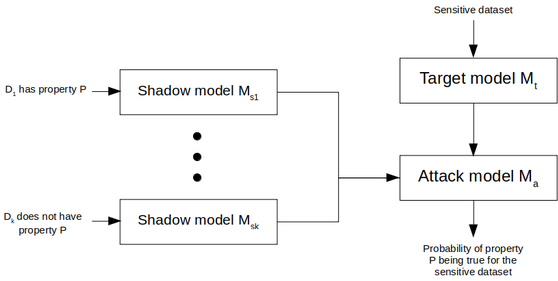
\includegraphics[width=0.99\textwidth]{pia_diagram2.png} % first figure itself
        \caption{Property Inference Attack using a meta-classifier and a dataset of shadow models.}
        \label{pia_diagram}
    \end{minipage}\hfill
\end{figure}

\section{Experimental Setup}

In this section, we describe the experimental settings: the dataset, the architectures of the target and attack models, and the evaluation metrics. The experiments were performed on a laptop with an Intel i7-8750H (2.20GHz) and 8GB RAM. The operating system is Ubuntu 20.04. The training of the shadow models and the attack models were both done using Pytorch and an Nvidia Quadro P600 GPU.\\

\subsection{Datasets}

CelebFaces Attributes (CelebA) \cite{liu2015faceattributes} is a face attributes dataset containing more than 200 000 images of more than 10 000 celebrities taken from online. The images are labeled using 40 physical attributes such as hair color, smiling, wearing a hat. We use the dataset to train the shadow models $M_s$ to detect whether the person has their mouth open using the \textit{Mouth\_Open} attribute. In the time of a COVID-19 pandemic, this attribute can be associated with someone not wearing a mask. Some companies are already marketing mask-detection software\footnote{https://www.theverge.com/2020/5/7/21250357/france-masks-public-transport-mandatory-ai-surveillance-camera-software}. The property targetted by the attacker is the gender proportion of the training set using the \textit{Male} attribute.\\

\subsection{Shadow Models}
The shadow models are trained to differentiate between images of persons with and without their mouth open.
However, the goal of the attacker is to infer whether the training set of a given model was composed of an unbalanced number of images representing males. The targetted property is a biometric data and is classified as sensitive data according to the GDPR. For a given model, the property $P$ can be formalized as follow: \textit{P is true when the training set of the model is composed of 70\% or more images containing males, otherwise, P is false}. It is important to note that $P$ is not related to the classification task of the model and that the target model does not use, at any time during training, the gender attribute.\\

The shadow models $M_{s_k}$ must have the same architecture as the targetted model, and be trained to a reasonable level of accuracy for the network to retain some information about the training set. For the attack to be effective, a large number of shadow models need to be trained. For each target model architecture, we constructed 1800 unique training sets of images from CelebA, one for each of the 1800 shadow models. The computational cost of such training is not negligible so we decide to lower it by reducing the size of the shadow datasets $D_{s_k}$ to 2000 different images each randomly selected from the test set of \textit{CelebA}. Out of the 1800 shadow models, 900  were trained on datasets presenting the property $P$ and 900 without. For each dataset, the exact proportion of males was randomly taken from a uniform distribution.\\

We trained several architectures based on the frame presented in Table \ref{shadow_architecture}. Each architecture has up to 3 convolutional layers each followed by a max-pooling layer with a ReLU activation, the second part of the network contains up to 3 fully connected layers with ReLU activation. The shadow models were trained using the Mean Squared Error loss and the Adam optimizer with a learning rate of 0.001 during 50 epochs.

\begin{table}[h]
\centering
\begin{tabular}{@{}ll@{}}
\toprule
Name              & Description       \\ \midrule
Convolution 1     & 6 filters 5x5     \\
Max-pool          & 2x2, ReLU         \\
Convolution 2     & 16 filters 5x5    \\
Max-pool          & 2x2, ReLU         \\
Convolution 3     & 32 filters 5x5    \\
Max-pool          & 2x2, ReLU         \\
Fully-Connected 1 & 120 neurons, ReLU \\
Fully-Connected 2 & 84 neurons, ReLU  \\
Fully-Connected 3 & 1 neuron          \\ \bottomrule
\end{tabular}
\caption{General frame for the architectures of the shadow models. }
\label{shadow_architecture}
\end{table}


\subsection{Attack Model and Evalution}
The attack model classifies shadow models as models trained on a dataset presenting the property $P$ or not. The dataset used is composed of the 1800 shadow models and is split into training (1500 shadow models), validation (100 models), and test sets (200 models). The attack model is a deep neural network that was tunned using the validation set and finally evaluated on the test set. The inputs of the attack model are the flattened weights of the model it is trying to classify as having the property $P$ or not. Therefore, a shadow model architecture with a larger number of parameters induces a wider input layer for the attack model. We created 10 attack models for each shadow model architecture and present the average performance across the 10 repetitions.\\

\begin{table}[h!]
\centering
\begin{tabular}{@{}ll@{}}
\toprule
Name              & Description       \\ \midrule
Fully-Connected 1 & 10 neurons, ReLU  \\
Fully-Connected 2 & 10 neurons, ReLU  \\
Fully-Connected 3 & 5 neurons, ReLU  \\
Fully-Connected 4 & 1 neuron          \\ \bottomrule
\end{tabular}
\caption{Architectures of the attack model. [TODO]}
\label{shadow_architecture}
\end{table}

\section{Results and Discussions}
Accuracies of the PIAs on each of the architectures of the target model are presented in Figure \ref{accuracies}. The larger/complex the target model is the more successful the PIA is. TODO

\begin{figure}[h!]
    \centering
    \begin{minipage}{\textwidth}
        \centering
        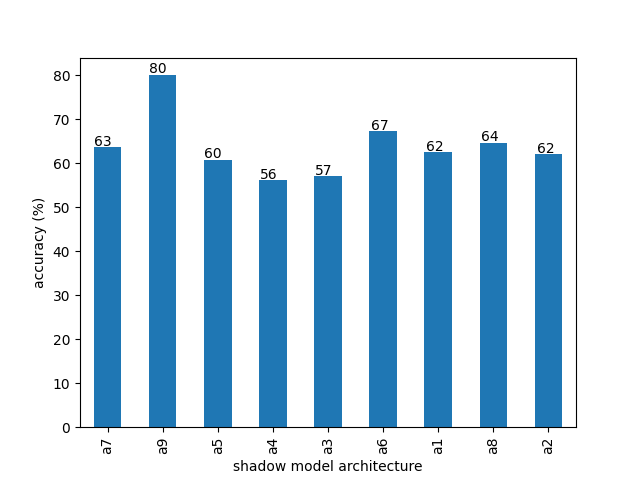
\includegraphics[width=0.99\textwidth]{accuracies.png} % first figure itself
        \caption{Accuracies of the attack of each architecture of target models. The architecture are ordered by increasing number of parameters.}
        \label{accuracies}
    \end{minipage}\hfill
\end{figure}

\newpage
%\renewcommand\bibliographytypesize{\small}
%\bibliographystyle{alpha}
%\bibliography{references.bib}{}
\bibliographystyle{unsrtnat}
\bibliography{references.bib}


\end{document}
